\section{Design choices }

In this section we present the reasons behind our implementation decisions for the design solutions shown in the Design Document.

\subsection{Data layer}


Due to our choice of Laravel as Backed Framework (\ref{backendchoice})  the available options as DBMS were the following:
\begin{itemize}
	\item MySQL
	\item PostgreSQL
	\item SQLite
	\item SQL Server
\end{itemize}
We chose to use \href{https://www.postgresql.org/}{postgreSQL} since its the only open-source of these solutions, apart from SQLite (which is not a client-server database engine and therefore does not suit our purposes).\\
Also postgreSQL is known for its reliability and ability to operate at scale.

\subsection{Business Logic Layer}

\subsubsection{External Services}
\label{exservices}
The external services are used in the application to retrieve information concerning available travel options and related travel times. This is done through the use of the \href{https://https://developers.google.com/}{Google Maps Directions}, \href{https://www.mapbox.com}{Mapbox} and \href{https://developer.uber.com/}{Uber} APIs.\\
The application also allows the user to book one of the available taxi option, provided by Uber service.\\
Furthermore, an external Mail service is used to send an email to the new registered User, in order to confirm the subscription to the application.

\subsubsection*{Google API}
This API allows the developer to search for directions for several modes of transportation, including public transportation, driving and walking.\\
The main use of this service is to retrieve available travel options between locations and related travel times.\\
The calls to the API are made with the use of an access token through an HTTP GET request built with cURL.\\
The request parameters includes the type of transportation requested, origin and destination coordinates, expressed as floating point latitude and longitude. The response is a JSON object which contains informations such as travel times and waypoints for directions.

\subsubsection*{Mapbox API}
This API, similarly to the previous one, allows the user to search for directions.\\
Their use in the application is due to the fact that Google API doesn't allows the developer to retrieve information concerning cycling mode of transportation.\\ 
Like before, the calls to the API are made with the use of an access token through an HTTP GET request built with cURL. The parameters of the requests are the origin and destination coordinates and the mean of transport, in this case we asked only for the cycling information. The response is a JSON object which contains informations such as travel times and waypoints for directions.

\subsubsection*{Uber API}
Uber is one of the widely used taxi service in the world. This API allows the User to book one of the available services provided.\\
This API are used in order to retrieve information concerning travel time about Uber services and then allowing the User to book one of the available options.\\
The call to the API are used for two different scopes:
\begin{itemize}
	\item \textbf{Retrieve travel options}\\
	For this operation, the calls to the API are made with the use of a server access token through an HTTP GET request built with cURL in which the parameters of the requests are the origin and destination coordinates.\\
	The response is a JSON object which contains travel options information.
	\item \textbf{Book a travel}\\
	In this case, the User has to login with his personal credential to the Uber platform. Once is logged in, the calls for the request of a booking are made with the personal access token of the User through an HTTP POST request built with cURL. The parameters of the request are the access token and the informations concerning the travel.\\
	The response is a JSON object which contains the booking information.
\end{itemize}

\subsubsection*{Mail Service}
The Laravel framework used to build the application, provides many methods to send mails. One of the most common, and the one implemented in the application, is the one in which Google Mail is used as mail server. 

\subsubsection{Framework}
\label{backendchoice}
For the Business Logic Layer we chose to implement our solution using the \href{https://laravel.com/}{\textbf{Laravel Framework}}.\\
Laravel is a free, open-source PHP web framework based on MVC, with an active and growing community behind it.\\
In this section we present the reasons behind this choice.

\subsubsection*{Language}
Laravel is a PHP based framework. PHP is a server scripting language and arguably one the most popular languages for back-end development.\\
Furthermore from the last version Laravel supports PHP 7 which offers remarkable improvements both in terms of performance and security.

\subsubsection*{Routing}
Laravel provides \textbf{routes management} out of the box.
It allows easy binding of the routes with the methods responsible for handling incoming requests.\\
It also allows to create routes for the managing of CRUD resources binding each HTTP method to the specified endpoint and to the corresponding methods, as shown in the table below.
\begin{figure}[H]
	\centering
	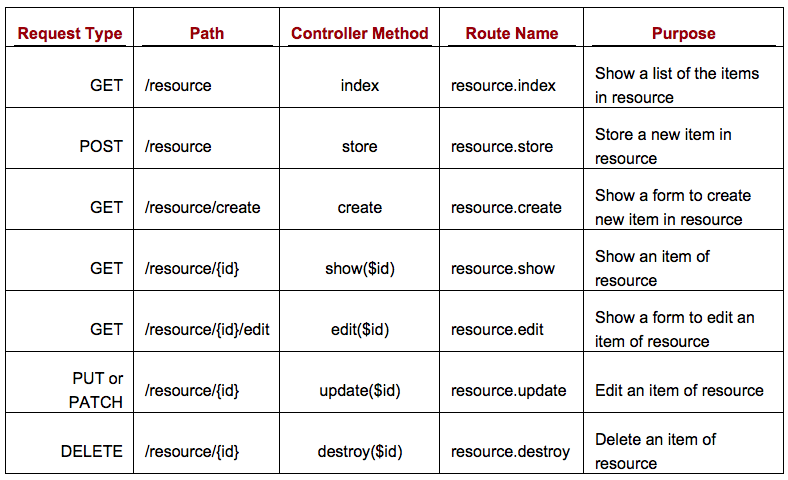
\includegraphics[scale=0.85]{crud}
	\caption{Laravel CRUD routing}
\end{figure}
\noindent Further details about the available routes and implemented APIs are in section \ref{rest}.

\subsubsection*{ORM}
Laravel includes among its default packages also \href{https://laravel.com/docs/5.5/eloquent}{\textbf{Eloquent ORM}}.\\
This package provides a simple ActiveRecord implementation for working with a database.\\
The active record pattern is an architectural pattern that stores in-memory object data in relational databases or as described by its creator: "An object that wraps a row in a database table or view, encapsulates the database access, and adds domain logic on that data.".\\
In Laravel each database table has a corresponding "Model" which is used to interact with that table, allowing to easily define relationships between different Models.\\
Further details about the Database and Model structure are in section \ref{dbmodel}

\subsubsection*{Database Management and Query Builder}
\label{dbmanagement}
Laravel provides a uniform way to interface with a variety of different DBMSs, it allows to design the database schema and migrate it on different DBMS solutions.\\
Furthermore Laravel's database query builder provides a convenient, fluent interface to create and run database queries.\\
It can be used to perform most database operations in the application and works on all supported database systems.\\
The Laravel query builder uses PDO parameter binding to protect against SQL injection attacks. 

\subsubsection*{Authentication}
Laravel only offers session based authentication out of the box.\\
For the development of APIs there is the need of a different type of authentication since there is no lasting session, for this reason we use an external package called \href{https://laravel.com/docs/5.5/passport}{Passport}, that easily integrates with Laravel.\\
Laravel Passport is an OAuth2 server and API authentication package that provides token based authentication.

\subsubsection*{Testing}
Laravel is built with testing in mind. In fact, support for testing with PHPUnit is included by default.\\
The framework also ships with convenient helper methods that allow you to expressively test your applications.
Along with the functionalities provided by the PHPUnit testing suite, Laravel allows to:
\begin{itemize}
	\item simulate an incoming request to an endpoint and the subsequent response.
	\item make assertions concerning the state of the Database.
	\item activate and deactivate the various middlewares (e.g. the authentication check or the active account check).
	\item choose the acting role (e.g. a specific account or privilege level).
	\item wrap each test function in a database transaction allowing each test to be independent.
\end{itemize}  

\subsection{Presentation Layer/Client}

\subsubsection{iOS}
For the presentation (front end) layer, we chose to develop a native iOS app for iPhones and iPads written in \href{https://developer.apple.com/swift/}{Swift}. 
We took this choice mainly for the widespread diffusion of the iOS operative system and for the several advantages of a native application, such as:
\begin{itemize}
	\item It is easier to work with and also performs faster on the device
	\item Provides full support from the App Store
	\item It is complete safe and secure
	\item Native look and feel
\end{itemize}

On the other hand, this choice leads to a loss in terms of portability and higher maintenance costs, as we do not have a common code base for different platforms.

\subsubsection{Swift}
Swift is a general-purpose, multi-paradigm, compiled programming language developed by Apple Inc. for iOS, macOS, watchOS, tvOS, and Linux. Swift is designed to work with Apple's \textit{Cocoa} and \textit{Cocoa Touch} frameworks and the large body of existing Objective-C  code written for Apple products. It is built with the open source LLVM compiler framework and has been included in Xcode since version 6.
\\ \\
Swift defines away large classes of common programming errors by adopting modern programming patterns:

\begin{itemize}
\item Variables are always initialized before use
\item Array indexes are checked for out-of-bounds errors
\item Integers are checked for overflow
\item Optionals ensure that nil values are handled explicitly
\item Memory is managed automatically
\item Error handling allows controlled recovery from unexpected failures
\end{itemize}

\subsubsection{External frameworks}
We used several external frameworks to accomplish what we stated in the RASD and DD document in a more elegant and secure way.
All the frameworks were installed with \textit{CocoaPods}, a dependency manager for Swift and Objective-C Cocoa projects. It has over 41 thousand libraries and is used in over 3 million apps.
\begin{itemize}
	\item \textbf{SWRevealViewController}: to add a slide-out side bar menu.
	\item \textbf{JTAppleCalendar}: to build a calendar from scratch and customize it for our needs.
	\item \textbf{SwiftDate}: to manage Dates and Timezones in Swift.
	\item \textbf{Alamofire}: to make elegant network HTTP requests.
	\item \textbf{CropViewController}: to perform basic manipulation on UIImage objects; specifically cropping and some basic rotations.
	\item \textbf{KeychainSwift}: helper functions for saving text in Keychain securely.
	\item \textbf{UberRides:} to integrate the Uber Rides API into our iOS app.
	\item \textbf{Quick/Nimble}: to help making asynchronous integration tests in a proper way.
\end{itemize}

\subsubsection{Apple frameworks}
In addition to all the external frameworks presented above, it is worth mentioning the adopted basic Apple frameworks:

\begin{itemize}
	\item \textbf{Foundation Kit}: provides a base layer of functionality for the app, including data storage and persistence, text processing, date and time calculations, sorting and filtering, and networking.
	\item \textbf{UIKit}: provides the required infrastructure for the app. It provides the window and view architecture for implementing the interface, the event handling infrastructure for delivering Multitouch and other types of input.
	\item  \textbf{MapKit}: to display map or satellite imagery directly from the app's interface, call out points of interest, and determine placemark information for map coordinates.
\end{itemize}

\subsubsection{Model View Controller}
Applications developed for iOS follow the MVC pattern.
The MVC design pattern assigns objects in an application to one of three roles: model, view, or controller. 

The pattern defines not only the roles objects play in the application, it defines the way objects communicate with each other. Each of the three types of objects is separated from the others by abstract boundaries and communicates with objects of the other types across those boundaries.

\begin{figure}[H]
	\centering
	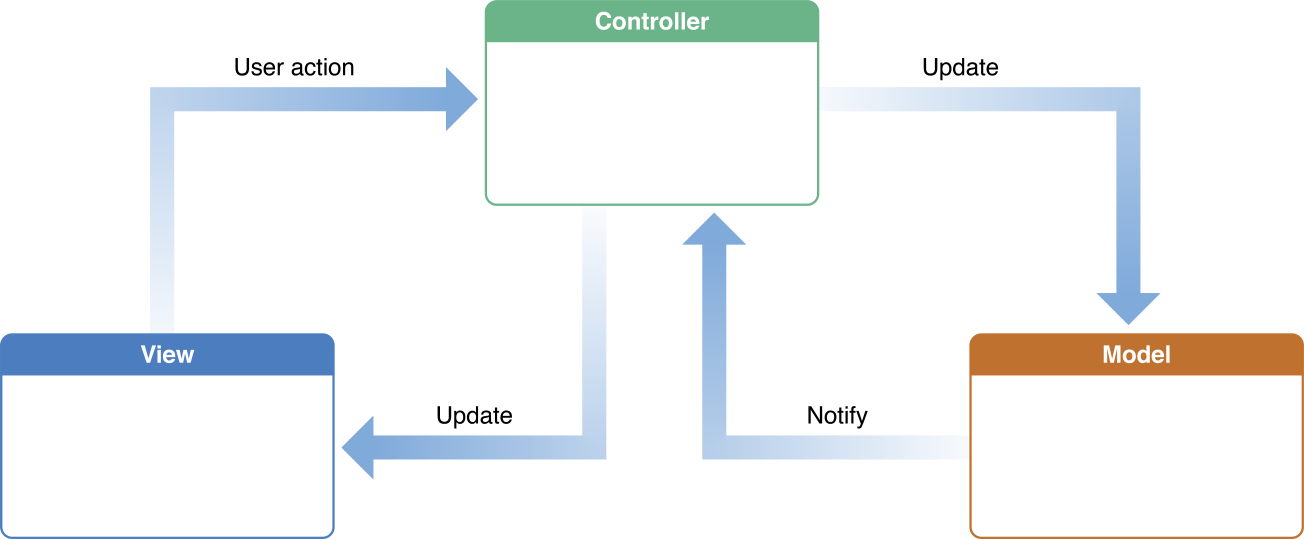
\includegraphics[scale=0.30]{mvc}
	\caption{Model View Controller schema}
\end{figure}

\begin{itemize}
	\item \textbf{Model:} model objects encapsulate the data specific to an application and define the logic and computation that manipulate and process that data.
	\item \textbf{View:} a view object is an object in an application that users can see. A view object knows how to draw itself and can respond to user actions. A major purpose of view objects is to display data from the application’s model objects and to enable the editing of that data.
	\item \textbf{Controller:}  controller object acts as an intermediary between one or more of an application’s view objects and one or more of its model objects. Controller objects are thus a conduit through which view objects learn about changes in model objects and vice versa.
\end{itemize}

\noindent
MVC roles played by an object can be merged. \textit{Travlendar+} widely uses \textbf{View Controllers}, controllers that concerns their selves mostly with the view layer. They “own” the interface (the views); their primary responsibilities are to manage the interface and communicate with the model.

